\documentclass[letter paper, 11pt]{article}
\usepackage{amsmath, enumerate, amssymb, amsthm, graphicx}
\usepackage[left = 1in, right = 1in, top = 1in]{geometry}

\title{CS 244 Project 3}
\author{Sweet Song(shihui) and Jason Zhao(jlzhao)}
\date{}

\begin{document}
\maketitle{}
\section*{Jellyfish - Networking Datacenter Randomly}
\subsection*{Introduction}


Jellyfish is a novel topology for organizing data center networks. Unlike traditional techniques such as Fat-trees and other well defined structures, Jellyfish proposes a random graph topology for top-of-rack switches. The authors show that this approach is both more cost efficient and can support more servers with the same amount of equipment. Furthermore, Jellyfish topologies can maintain the same overall throughput as Fat-tree networks due to short average path length between nodes.

\subsection*{Background and Results to Reproduce}


Jellyfish uses a simulated random regular graph(RRG) to wire up top-of-rack switches in a data center network. The RRG algorithm simply add links between 2 random non-neighboring switches until there are no open ports remaining. In the case where there are still open ports but no links can be added, an existing link can be removed and the algorithm will proceed. This graph structure exhibits low average path length between servers. Consider the following figure,

\begin{center}
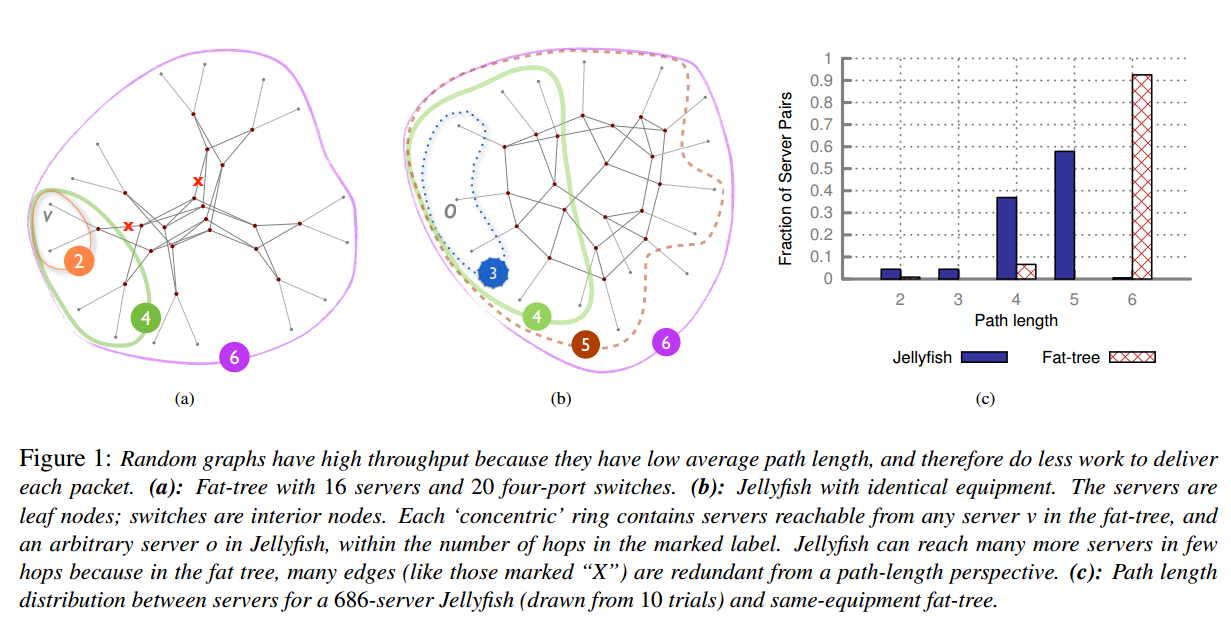
\includegraphics[scale=0.4]{jellyfish}
\end{center}

Most nodes in a Fat-tree network are 6 hops apart whereas in Jellyfish, most nodes are between 4-5 hops apart. Not only are paths shorter in Jellyfish, the RRG network also has more distinct paths between end hosts. This improves the fault tolerance of the overall network but requires different routing algorithms in order to maximize the benefits. We aim to reproduce the following figure from the original paper

\begin{figure}
\centering
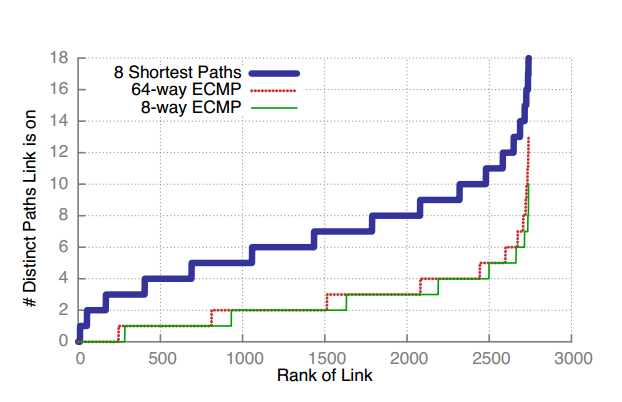
\includegraphics[scale=0.5]{9}
\caption{Figure 9 from the Jellyfish paper. ``ECMP does not provide path diversity for Jellyfish: Inter-switch link's path count in ECMP and k-shortest-path routing for random permutation traffic at the server-level on a typical Jellyfish of 686 servers (built using the same equipment as a fat-tree supports 686 servers). For each link, we count the numbre of distinct paths it is on. Each network cable is considered as two links, one for each direction.''}
\end{figure}

This figure shows that in order to fully maximize the path diversity in Jellyfish, traditional multi-path routing algorithms such as equal-cost multi path routing (ECMP) is not sufficient. Over 50\% of links are only on 2 or fewer distinct paths between servers where as in k-shortest path routing, only around 6\% are on 2 or fewer distinct paths. With newer TCP modes such as multi-path TCP, having more distinct paths can significantly increase the throughput of the sending server. We hope to replicate this experiment and verify that ECMP does in fact produce fewer distinct paths compared to the k-shortest path routing algorithm.

\subsection*{Methods}


We first generated a random regular graph with n servers and k ports per server. To closely approximate the topology as stipulated in figure of the paper, we created a python script $genGraph.py$ to spawn this for a total of 220 switches with 12 ports each. Then $traffic.py$ randomly assigned 686 servers to each switch with uniform probability. The traffic script then creates a random permutation traffic matrix where each server is sending to exactly 1 other server and receives from
exactly 1 other server. This traffic matrix is then passed to $genPaths.py$ to calculate the number of available path for each flow. To compute the paths, we used BFS to find $k$ shortest paths from one end point to another. The same algorithm is used to compute the available paths for ECMP where the cost metric is simply number of hops. We then aggregated the number of time each link is used for the following 3 algorithms: 8-shortest paths, 8-way ECMP, and 64-way ECMP.
Finally, the links were ranked by the number of distinct paths they are on and this was plotted using gnuplot.

This result is reproducible on any machine with python 2.7+ and gnuplot installed.
\subsection*{Outcome}


\begin{figure}
    \centering
    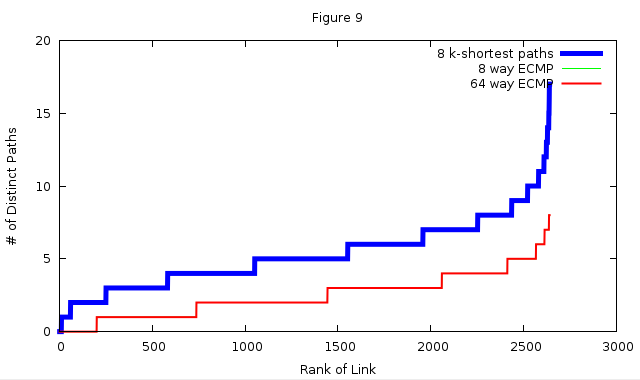
\includegraphics[scale=0.5]{outcome}
    \caption*{Figure 9 reproduced using our own RRG and path finding algorithms.}
\end{figure}
To our delight, our plot looks almost identical to the plot of the graph. The step functions in our output mimic those in the graph, with some rank differences. The range of the graph also closely resembles the original papers. The minor differences between where the step occurs can be attributed to the randomness in the graph generation. One interesting thing to note is that since the original topology is not well defined, the actual graph can be very different depending on the
characteristics of the switches being used. For example, if we used fewer switches with more ports per switch, the number of distinct paths will decrease because there are fewer nodes in the network. We plan on varying this experiment with different graph characteristics.

\subsection*{Issues}


The vagueness of the topology for the plot was a hindrance during our development. In particular, there was no mention of number of ports per server. Deducing backwards from the ~2600 rank of link graph, we concluded that the number used in the simulation was most likely 12. Another problem that arose was the absolute similarity between our 8-way EMCP and the 64-way EMCP number of distinct paths the links were on. That is, there were always only 8 or less shortest paths between
every pair of source and destination that had the same lowest weight. We will continue to investigate this issue for the final blog post.

\subsection*{Future Direction}
We are very confident in the reproducibility of figure 9, for the final blog post, we will very the random graph with different switches to see if there is a large variation in distinct paths. We also plan on running an actual throughput simulation using a Jellyfish network and a Fat-tree network in Mininet if possible. Since running a full scale simulation requires a lot of code, we hope to get some existing ECMP and MPTCP code from the TAs and assess how much work it will
be.

\end{document}
